\chapter{Estado de la cuestión}

\section{Introducción}

En este capítulo, se da cuenta de la importancia de la enseñanza de las ciencias de computación en la escuela media, señalando cómo la robótica puede servir de herramienta para lograr ese cometido, aprovechando sus particularidades y ventajas a la hora de abordar conceptos propios del pensamiento algorítmico (repeticiones, recursividad, saltos condicionales). Estos planteos se encuentran en consecuencia con la actual ley Nacional de Educación N\grad 26.206 que, en su artículo 30\grad, Inc. F, enuncia: 

\textit{Desarrollar  las  capacidades  necesarias  para  la  comprensión  y  utilización  inteligente  y  crítica  de  los  nuevos  lenguajes  producidos  en  el  campo  de  las tecnologías de la información y la comunicación.}

Podemos decir, que las ciencias de la computación \citep[pág 4]{sadosky2013cc} se volverán de vital importancia a la hora de pensar un esquema curricular específico para abordar los contenidos básicos propuestos por dicha ley.

\section{Antecedentes}

\subsection{Lenguaje LOGO}
El uso de dispositivos robots para enseñanza, tiene su origen en el ya referido trabajo de Seymour Papert, y su desarrollo del lenguaje LOGO. Este lenguaje formal \citep{giro_lenguaje_2015} fue diseñado para trabajar conceptos de matemáticas y geometría mediante la interacción con un robot con forma de tortuga (de ahí que el logotipo de LOGO sea una tortuga). Este dispositivo se movía sobre una superficie plana dibujando en función de las instrucciones previamente creadas en una computadora. Basado en ese esquema, los discentes programaban en lenguaje LOGO (un lenguaje muy parecido en su forma al lenguaje LISP), luego activaban el robot tortuga y la computadora enviaba las órdenes para que éste se mueva, dibujando sobre un papel. 

A través de esa experiencia, Papert colabora con la empresa LEGO para fabricar el producto LEGO\textsuperscript/LOGO, el cual después pasaría a ser conocido como LEGO MINDSTORM\textsuperscript{\texttrademark}, una plataforma física basada en fichas LEGO\textsuperscript{\textregistered} que también incluye hardware de adquisición de datos capaz de leer sensores y trabajar sobre diversos actuadores.

Con el tiempo, el lenguaje LOGO abandonaría la tortuga robot. El elevado costo de cada robot tortuga y el abaratamiento de las micro computadoras (por ej. COMMODORE\textsuperscript{\textregistered} c64) con capacidad de procesar gráficos a color  hicieron que fuera muy difícil implementar una currícula basada en LOGO solamente usando elrobot tortuga.

\begin{figure}[htb]
  \begin{center}
    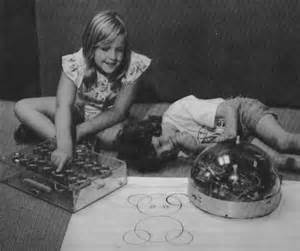
\includegraphics[width=0.5\textwidth]{figuras/logo_robot.jpg}
    \caption[Caption for LOF]{robot 'tortuga' original diseñado por el M.I.T}
    
    \label{fig:tortuga_mit}
  \end{center}
\end{figure}

El lenguaje LOGO está diseñado para ser sencillo de aprender, con instrucciones ''primitivas'' (en el argot LOGO) que son intuitivas para el usuario; la palabra 'adelante', hace que la tortuga avance N pasos,  al igual que ''atrás'' hace que retroceda. Sin embargo sigue siendo un lenguaje de programación completo y capaz de hacer lo mismo que otros lenguajes de propósito general  (como C, FORTRAN u otros lenguajes de la época). 

Una de las ventajas de LOGO es su facilidad de poder hacer ''algo'' con muy pocas lineas de código (típicamente algún dibujo con la ''tortuguita''), \cite{seymour_papert_desafio_1987} plantea que cualquier niño, bajo las condiciones adecuadas, puede aprender un lenguaje de programación como LOGO.

Originalmente, las primeras pruebas de LOGO se hicieron con robots como el de la figura \ref{fig:tortuga_mit}, el cual estaba pensado para ser robusto, y capaz de soportar hasta el peso de un niño encima. Las computadoras de la época no tenían capacidad de procesar gráficos de alta definición (y las impresoras eran caras y de uso casi exclusivo en las empresas), por lo tanto la ventaja de disponer de un robot que dibuje eran muy atractivas.

\begin{figure}[htb]
  \begin{center}
    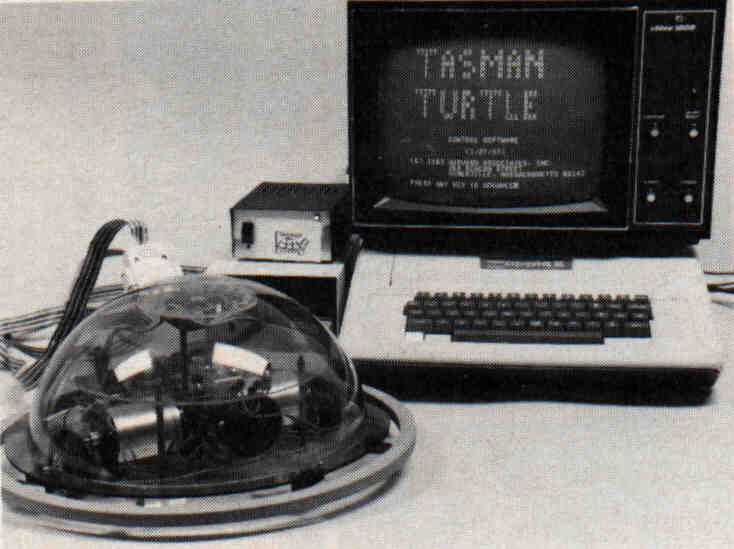
\includegraphics[width=0.5\textwidth]{figuras/turtle_with_apple.JPG}
    \caption[Caption for LOF]{Versión 'mini' del robot tortuga controlado por un micro computador Apple}
    
    \label{fig:tortuga_2}
  \end{center}
\end{figure}

Con el advenimiento de las micro computadoras (como las ZX spectrum\textsuperscript{\texttrademark}  y las commodores\textsuperscript{\texttrademark} C64), que contaban con la capacidad de trabajar  en monitores a color (o en los televisores CRT de la época) tenian bajo costo de adquisición, se dejó de utilizar a los robots tortuga, para directamente trabajar con el lenguaje de programación LOGO y una ''tortuga virtual'', menos llamativa pero mucho mas barata de adquirir para los colegios. 

\subsection{ARDUINO\textsuperscript{\texttrademark} y la revolución del hardware libre.} 


El primer modelo de la placa Arduino\textsuperscript{\texttrademark} fue introducido en 2005, ofreciendo un bajo costo y facilidad de uso para novatos y profesionales. Buscaba desarrollar proyectos interactivos con su entorno mediante el uso de actuadores y sensores. Su bajo costo y la enorme cantidad de documentación generada por las distintas comunidades de desarrolladores y entusiastas permitió que la plataforma Arduino\textsuperscript{\texttrademark} se volviera un estándar a la hora de hablar sobre automatización o IOT (Internet of things).

Actualmente los miles de kits para enseñanza de robótica que se diseñan y fabrican (a pequeña o gran escala) están basados en la arquitectura Arduino\textsuperscript{\texttrademark} y la serie de micro controladores AVR\textsuperscript{\textregistered} de 8 bits. La inmensa documentación disponible y la facilidad de adquisición de los componentes, ha expandido su uso por parte de diversas comunidades y con diversas finalidades, entre ellas, la enseñanza de robótica. Esta gran demanda,  también incidió en el abaratamiento de los costos de fabricación del hardware. Los kits generalmente constan de una serie uniforme de componentes electrónicos y mecánicos, como servo motores, motores de corriente continua, sensores analógicos / digitales y componentes de electrónica discreta (resistencias, leds, capacitores, entro otros), que permiten trabajar una serie de sistemas de automatización, robótica y/o domótica de mayor o menor complejidad.

\begin{figure}[htb]
%{R}{0.5\textwidth}
  \begin{center}
    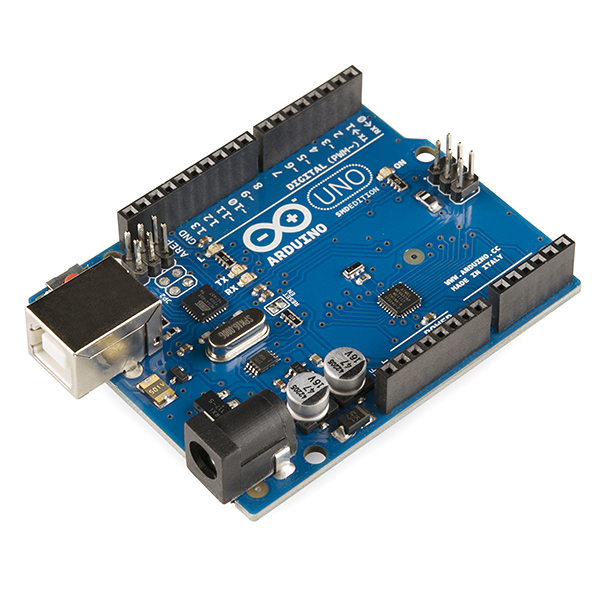
\includegraphics[width=0.5\textwidth]{figuras/Arduino_Uno_-_R3.jpg}
    \caption[Caption for LOF]{Arduino\textsuperscript{\texttrademark} Uno Rev. 3}
       
   \label{fig:arduinouno }
  \end{center}
\end{figure}

%\texttrademark : pone el símbolo TM
%\textregistered : pone el símbolo consistente en una R rodeada de un círculo
%\textcopyright : pone el símbolo consistente en una C rodeada de un círculo
\section{lenguajes de programación en la enseñanza}

En la actualidad y en el marco de la ley Nacional de educación, la enseñanza de la ciencia computacional está tomando relevancia a nivel curricular. La falta de profesionales especializados en programación y la constante demanda de ''mano de obra'' por parte de la industria del software (software factory) se ha vuelto un factor de preocupación por parte de las autoridades nacionales. Para tratar de paliar esa problemática, se están implementando distintos planes y programas gubernamentales. Dentro de estos proyectos podemos encontrar el Programa \textbf{Escuelas del Futuro}, situado en la órbita de la Secretaría de Innovación y Calidad Educativa del Ministerio de Educación y Deportes de la Nación. El mismo busca: 

\begin{center}
\textit{
crear un Proyecto con el objeto de generar un cambio transformador en las estrategias pedagógicas y políticas de contenidos para integración del sistema educativo a la cultura digital.
Que para el logro de los objetivos previstos en los considerandos precedentes, resulta conveniente la creación del Proyecto ''Escuelas del Futuro'' orientado a propiciar alfabetización digital de todos/as los/as estudiantes de la Argentina, a través de integración de áreas de conocimiento emergentes, como la programación y la robótica. \footnote{Resolución Ministerial 2.376/16 Ministerio de Educación y Deportes, consultado en http://www.saij.gob.ar/proyecto-escuelas-futuro-nv15957-2016-12-05/123456789-0abc-759-51ti-lpssedadevon?}
} 
\end{center}

Desde esa perspectiva, y como señalan desde la Fundación Sadosky, la alfabetización digital parte de la enseñanza de la ciencia computacional  pensada como un conjunto amplio de fundamentos y principios independiente de tecnologías  \citep[pág 12]{sadosky2013cc} que incluyen:

\begin{enumerate}
  \item Programación y algoritmos
  \item Estructuras de datos
  \item Arquitecturas y redes de computadoras
\end{enumerate}

La ciencia computacional permite fomentar habilidades que pueden ser aplicadas a variados campos de estudio como:

\begin{enumerate}
  \item Modelización y formalización.
  \item Descomposición en sub problemas.
  \item Generalización y abstracción de casos particulares.
  \item Proceso de diseño, implementación y prueba.
\end{enumerate}

De esta forma, la enseñanza de un lenguaje formal toma una particular relevancia dentro del esquema educativo actual, que busca resolver los problemas planteados por la necesidad de alfabetizar digitalmente a la población.

Sin embargo, hay críticas concretas a la enseñanza del ''pensamiento algoritmico'' en contraposición a la enseñanza de lenguajes formales específicos. La idea de pensamiento algorítmico es que se pueden aprender conceptos de programación a través de meta-lenguajes, o lenguajes pedagógicos (pseudo código o sistemas basados en diagramas y gráficos). Desde esta perspectiva, un lenguaje educativo permitiría simplificar el contenido técnico complejo, y abordar de forma escalonada el aprendizaje de la ciencia computacional.

Como crítica a ese modelo, \cite{dijkstra2010que} plantean que la ''simplificación'' de un lenguaje formal con pseudo código o con lenguajes ''de juguete'' (como el caso del lenguaje BASIC en su momento), puede ser contraproducentes para el aprendizaje. En terminaos del propio Dijkstra:

\begin{center}
\textit{Es prácticamente imposible enseñar una buena programación a los estudiantes que han tenido una exposición previa a BASIC: como programadores potenciales son mentalmente mutilados más allá de la esperanza de regeneración.}
\end{center}[Traducción propia]

Para \cite{seymour_papert_desafio_1987}, los lenguajes simplificados como BASIC (o como los lenguajes basados en bloques gráficos de más reciente aparición) que se  ''promocionan'' como lenguajes simples de aprender a causa de su reducido vocabulario, son sin embargo, extremadamente complejos de usar para crear programas no triviales. El fenómeno del lenguaje BASIC fue definido por \cite{seymour_papert_desafio_1987} como el ''fenómeno QWERTY'', a causa de los teclados, que fueron diseñados en la época de las primeras máquinas de escribir mecánicas. Estas máquinas solían trabarse si se ponían cerca las teclas de uso más común; por ello, se diseñó un sistema de ordenamiento de letras denominado QWERTY que dificultaba la digitación veloz para evitar dicho problema. Aun después de la creación de las computadoras, cuando los problemas mecánicos de las máquinas de escribir ya no tenían sentido, se continuó usando ese mismo sistema. 

El caso de los  sistemas BASIC, sucedió algo similar: fueron diseñados para resolver problemas presentados por las primeras micro computadoras, simplificando su set de instrucciones. Una vez que esos problemas fueron resueltos por hardware más potente y de menor costo, la industria no obstante siguió eligiendo BASIC como herramienta de desarrollo y enseñanza de programación. 

% \begin{wrapfigure}{R}{0.5\textwidth}
%  \begin{center}
%    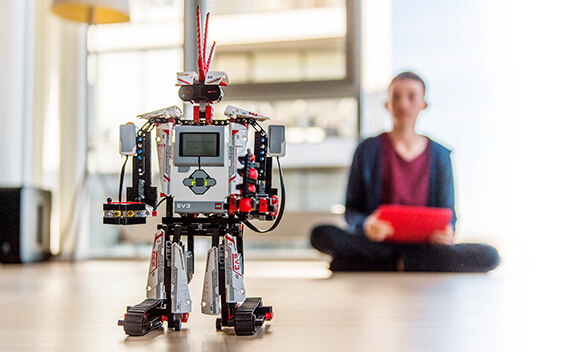
\includegraphics[width=0.5\textwidth]{figuras/lego_mindstorm.jpg}
%    \caption[Caption for LOF]{Robot LEGO\textsuperscript{\textregistered} MINDSTORM\textsuperscript{\textregistered}}
%    \label{fig:legomindstorm }
%  \end{center}
%\end{wrapfigure}

\subsection{Competencias especificas para el aprendizaje de un lenguaje de programación}

Para usar un lenguaje de programación (entendiendo este como un lenguaje formal de tipo especifico) como herramienta de enseñanza, es necesario tener en cuenta una serie de capacidades o características para que puedan ser incluidos en una currícula educativa. En general podemos decir, que un lenguaje de programación debería tener las siguientes cualidades:

\begin{enumerate}
   \item Ser de alto nivel (similar a un lenguaje natural).
   \item Ser un lenguaje de propósito general (la capacidad de crear cualquier programa).
   \item Tener capacidad multi paradigma (programación orientada a objetos, programación estructurada, etc.).
   \item Ser multi plataforma (capacidad de adaptarse a distintos dispositivos).
 \end{enumerate} 
 
También, es importante que un lenguaje de programación seleccionado para trabajar en el aula sea de uso común y extendido en la industria, no tanto por su éxito comercial momentáneo, que puede variar en muy poco tiempo, si no por la capacidad de conseguir documentación especifica y comunidades de soporte que permitan desarrollar al máximo las capacidades intrínsecas de la herramienta.

Hay que hacer una aclaración respecto a los lenguajes de marcado (como HTML), que no son lenguajes de programación propiamente dicho dado que no tienen características básicas como:

\begin{itemize}
   \item variables
   \item repeticiones
   \item sentencias condicionales
   \item recursividad
 \end{itemize} 

Si bien esta enumeración de características no es exhaustiva, pone en manifiesto que, habiendo una enorme cantidad de lenguajes de programación, algunos de características mas especificas que otros, la elección del lenguaje de programación que se usará para un curso de enseñanza inicial no es un asunto trivial.


\section{La robótica y la enseñanza de programación}

En la actualidad, el uso de robótica se está extendiendo dentro de los espacios curriculares, los robots educativos se presentan como una alternativa interesante para poder trabajar conocimientos transversales a distintas disciplinas, desde la matemática y programación hasta las ciencias naturales. No obstante, se podría decir que dónde más se pueden aprovechar las ventajas de los kits de robótica que pululan en el mercado es precisamente en la enseñanza de los lenguajes de programación.

Básicamente un robot es una computadora con sensores y actuadores que le permiten interactuar en un entorno físico; para lograr ese cometido el robot debe ser programado con un algoritmo que le permita resolver las situaciones complejas que pueden ocurrir mientras se mueve por un medio ambiente físico. A diferencia de lo que ocurre en un entorno virtual como un simulador robótico, interactuar en un espacio físico obliga al diseñador del algoritmo a tomar medidas de corrección y control mediante sensores, y dotar al robot de cierta ''inteligencia'' para resolver situaciones inesperadas, como fallas mecánicas o defectos de fabricación. Esto ultimo sobre todo cuando se usan componentes reciclados o de baja calidad.

Es importante hacer una distinción entre ''aprendizaje DE robótica '' y ''aprendizaje CON robótica'' \citep{malec2001some}, entendiendo que la robótica es una disciplina en sí misma, y su uso en la industria tiene un nivel de complejidad que requiere un grado de especialización extra para los técnicos e ingenieros que trabajen en ese ámbito. Por eso mismo el aprendizaje CON robots, debería ser pensado como un medio para facilitar la construcción por parte de los discentes de conocimientos transversales adaptando las complejidades inherentes al diseño y construcción de un robot. Este aprendizaje CON  promueve en los estudiantes el desarrollo de competencias tales como: la toma de decisiones basadas en
el conocimiento, el formular explicaciones científicas y el trabajo en equipo \citep{lopez2013aprendizaje}.
